\section{Introduction}
\label{section:intro}

Datacenter networks must support an increasingly diverse set of
workloads.
Small latency-sensitive flows to support real-time applications such
as RPCs share the network with large
throughput-sensitive flows for big data analytics or VM
migration.
Load balancing the network is crucial to ensure operational efficiency
and suitable application performance.
Unfortunately, popular flow-hashing-based load balancing schemes,
\eg{}, ECMP, cause congestion when hash collisions
occur and
perform poorly in asymmetric topologies.
A variety of load balancing schemes aim to address the
problems of ECMP. Centralized schemes
% such as Hedera~\cite{hedera} and
%Planck~\cite{planck}
% collect network state and reroute elephant flows
%when collisions occur.
%These approaches 
are reactive and very coarse-grained due to the large time constants of their control
loops or require extra network
infrastructure~\cite{planck}.
Transport layer solutions such as MPTCP~\cite{mptcp}, can
react faster but require widespread adoption and are difficult to
enforce in multi-tenant datacenters.
%Also, our experiments in Section~\ref{sec:micro}, ~\ref{sec:eval} and 
%CONGA~\cite{conga} show MPTCP has brittle performance in many workloads. 
In-network reactive distributed load balancing schemes, \eg{},
CONGA~\cite{conga}, can be
effective but require specialized networking hardware.
%~\cite{conga,juniper-vcf,detail,packetspray}.
%NOTE: where does Mahout go? DCTCP?

%The design of above schemes ignore recent trends in datacenter network design. Complex newtork
%hardware leads to extra cost, vendor lock-in, and increased down-time. 

\section{Our Approach}

%The shortcomings of the above approaches cause us to re-examine the design space for load balancing in datacenter networks. ECMP, despite its limitations, is a highly practical solution due to its proactive nature and stateless behavior.
%It provides clear benefits in robustness and simplicity 
%compared to the complex and often fragile reactive schemes. 
%Conceptually, ECMP's flaws are not internal to its operation but are caused by asymmetry in network topology (or capacities) and variation in flow sizes. {\em In a symmetric network topology
%where all flows are ``mice'', ECMP should provide near optimal load balancing}; indeed, prior work~\cite{conga,flowlet} has shown the traffic imbalance ECMP imposes across links goes down with an increase in the number of flows and a reduction in the variance of the flow size distribution. 

%Can we design a good proactive load balancing scheme without requiring special purpose hardware or modifications to end-point transport? 
%The system we propose relies on the datacenter network's {\em software edge} to transform arbitrary sized flows into a large number of near uniformly sized small sub-flows, and to proactively spread those uniform data units over the network in a balanced fashion. Our scheme is fast (works at 10+ Gbps), and doesn't require network stack configurations that may not be widely supported outside the datacenter (such as increasing MTU sizes). We piggyback on recent trends where several network functions are moving into hypervisors and software virtual switches on end-hosts~\cite{nv-mtd}. 
%Our paper makes a strong case for moving network load balancing functionality out of the datacenter network hardware and into the software-based edge.

% we really need expensive (and often fragile) congestion-aware reactive techniques like~\cite{hedera,mptcp,conga} to achieve load balancing in datacenter networks, or can we achieve a similar level of functionality by
% %1) adding symmetry to network 
% We argue that it is practical, cheaper, robust, and more efficient to do the latter. 

%It is important that such schemes not require any changes to the transport
%layer, extra network infrastructure or expensive network switches. 
\iffalse
Fortunately, many commonly deployed network topologies like 2-tier folded Clos (leaf-spine) already meet the network symmetry 
requirements though asymmetry may occur due to failures and should be handled. The main challenge then is to achieve uniformity 
in flow sizes i.e. a mechanism that can efficiently multiplex and de-multiplex logical flows into a more uniformly sized smaller 
sub-flow units. This mapping and the load balancing of the resulting units should ideally be done 
in the network itself instead of transport layer.
\fi
%We design our system to load balance arbitrary sized flows as near uniformly sized sub-flow units. 

%\aditya{this para can go - In the design of such a system, we draw 
%inspiration from network virtualization~\cite{nv-mtd,ovs-extending} and similar recent trends where several network functions (e.g. distributed firewall) 
%are being moved to the soft edge. We claim that hypervisors and soft virtual switches at the network edges are the ideal places to 
%implement the load balancing logic. Schemes like CONGA~\cite{conga} and Juniper VCF~\cite{juniper-vcf} aim to load balance in the "fabric", but
%ignore the fact that in many commercial datacenters, the {\em soft-edge} (\eg{} Open vSwitch~\cite{ovs-website}) is increasingly part of the 
%fabric as well~\cite{nv-mtd}.}

%See Nicira's NSDI 2014 paper~\cite{nv-mtd}. Conga's notion of fabric extends just to the leaf switches.


% The main thesis of this paper is to answer whether {\em fine-grained, non-reactive, near-optimal load balancing is implementable
% at the soft-edge}~\keqiang{better to say pro-active?}. Our design goals are that the system should not require changes to networking hardware or 
% additional networking infrastructure. Furthermore, the design should not require changes to the transport layer or complex transport 
% layer tuning. Finally, 

%
%the Fabric paper~\cite{casado2012fabric}, which advocates for a combined intelligent
%(software?~\keqiang{Yes, Fabric paper wrote "at present much edge forwarding in datacenters is done in software 
%by the host's general-purpose CPU", last page, second paragraph (top left)}) network edge with a simple label-switched core. 
%
%

\iffalse
Several challenges arise when employing the edge to load balance the network
on a sub-flow level. Software is slower than hardware, so operating at 10+ Gbps speeds means
algorithms must be simple, light-weight, and take advantage of optimizations in
the networking stack and offload features in the NIC. Any sub-flow level load balancing should also be 
robust against reordering.
%Due to variations in the end host networking stack~\cite{bullettrains},
%obtaining the "ground truth" of packet timing characteristics on the wire is difficult~\keqiang{vSwitch is below TCP/IP, 
%so what vSwitch observes is close to "groud truth". Undertand that you want to make a soft argument on flowlet here}. 
%We show flowlet-based
%load balancing schemes can be difficult to implement and tune in software, and therefore we must find an alternative
%approach to load balance the network while being robust against reordering. 
As shown in Section~\ref{sec:background}, 
reordering not only impacts TCP's congestion control mechanism, but also imposes significant computational
strain on hosts, effectively limiting TCP's achievable bandwidth if not properly controlled. Last, the approach must be 
resilient to hardware or link failures and be adaptive to network asymmetry.

\fi
%On the other hand, an open, software-based approach
%prevents extra hardware cost and vendor lock-in, and allows for simplified network management. These issues
%are cited as major concerns today (cite FB interview).
%Thanks to projects like Open vSwitch, soft-switching platforms are fast, mature, open source, adapted widely, remotely
%configurable, SDN-enabled, and feature-rich~\cite{nv-mtd}. Last, an intelligent soft-edge architechture
%is designed to be flexible and easily evolvable~\cite{casado2012fabric}.

% XXX - maybe we can argue something about cost: we need less over-subscription because we don't have to worry about burst/collisions/congestion as much.
% FB, for example, has 10 to 40 Gbps links (google altoona).
%Flexible: simplified core with software edge is evolvable. Consistent-updates~\cite{shadow-mac}.
%Soft-switching in end-hosts is already very mature and feature-rich,
%and some very sophisticated actions can be taken there. We're piggy-backing on this trend.
%
%{ \em If we arrive at a point where the edge processing is done in software
%and the core in simple hardware, then the entire infrastructure
%becomes much more evolvable} ---Martin Casado et al.~\cite{casado2012fabric}
%
%~\keqiang{found a good argument made in Shadow MAC paper, copied below}
%A recent position paper by Casado et al.~\cite{casado2012fabric} suggests that 
%next-generation networks should combine an intelligent network edge with a label-switched core. 
%Casado et al. arrive at this conclusion based on separating the concerns of end points, switches, and operators. 
%We arrive at the same conclusion based a different line of reasoning, which lends credence to the notion that 
%SDN-enabled networks should be architected in this fashion.
%
%Challenges: End-host overheard/impact on apps; keeping up with 10G speeds; solving packet reordering without touching transport layer;
%resilient to hardware or link failures, adaptive to network asymmetry.

We piggyback on recent trends where several network functions are moving into hypervisors and software virtual switches on end-hosts and advocate to move network load balancing functionality out of the datacenter network hardware and into the software-based edge, \ie{}, utilize vSwitches to break flows into discrete units of packets, called 
{\em droplets}, and distribute them evenly 
to near-optimally load balance the network. 
It uses the maximum TCP Segment Offload (TSO) size (64 KB) as droplet granularity, 
allowing for fine-grained load balancing at network speeds of 10+ Gbps.  
%Flowcells
%are near uniform in size because they are mostly independent of traffic patterns at the sender and 
%provide a natural interface to offload optimizations provided in the NIC and OS, allowing
%for fine-grained load balancing to scale to network speeds of 10+ Gbps. 
%Pushing the limits of fine-grained load balancing in fast networks means that reordering 
%must be addressed, 
%and therefore 
%To combat reordering, we modify the Generic Receive Offload (GRO) handler
%in the hypervisor OS to mitigate the computational burden imposed by reordering
%and prevent reordered packets from being pushed up the networking stack.
Reordering can cause TCP throughput degradation and impose significant computational burden by causing the Generic Receive Offload (GRO) handler to export many small segments. Our approach mitigates these problems by modifying GRO to ensure that large, in-order segments are pushed up to higher layers of the networking stack.
Finally, our system load balances the network
in the face of asymmetry and failures using a combination of fast failover and weighted multipathing at the network edge.

%with input from a centralized controller, vSwitches in Presto can load balance the network
%in the face of asymmetry, without requiring detailed global information about the 
%network topology or traffic patterns at each vSwitch.
%Presto can improve throughput, latency and fairness in the network and reduce mice flow completion
%time tail latencies.

\iffalse
Our paper makes the following contributions:
\begin{enumerate}

\item We design and implement a system, called Presto, that near-optimally load balances
links in the network. We show that such a system can be built with no changes to the transport
layer or network hardware, and scales to 10+ Gbps networking speeds.
%Presto  
%improves throughput, latency and fairness in the network and reduces flow completion time tail latencies
%for mice flows.
%\item We show that such a system can be built with no changes to the transport
%layer or within network hardware. Unlike previous approaches with similar design goals~\cite{drb}, we 
%ensure our approach scales to network speeds higher than 1 Gbps.
Our approach makes judicious use of middleware
already implemented in most hypervisors today: Open vSwitch and the TCP receive offload engine in the OS
(Generic Receive Offload, GRO, in the Linux kernel).\footnote{Also known as Receive Segment Coalescing (RSC)~\cite{ms-rsc}, or in hardware, Large Receive Offload (LRO)~\cite{grossman2005large}} 

%We show our approach can work in both SDN and non-SDN environments.
\item We uncover the importance of GRO on performance when packets are reordered.
At network speeds of 10+ Gbps, current GRO algorithms are unable to sustain line rate under 
severe reordering due to extreme computational overhead, and hence 
per-packet load-balancing approaches~\cite{drb,packetspray} need to be reconsidered. We
improve GRO to prevent reordering while ensuring computational overhead is limited.
%Our scheme can distinguish loss from reordering and adapt to prevailing network conditions.
%These techniques are criticial to ensure we minimize the time waiting for lost packets, while
%being robust against exposing reordering to higher network layers.  
We argue
GRO is the most natural place to handle reordering because it can mask
reordering in a light-weight manner while simultaneously limiting CPU overhead by having a direct impact
on the segment sizes pushed up the networking stack.
%Need to sell this more: this is the only place we should really do it because it has
%direct impact on packet sizes, and thus CPU overhead. We also need to talk about mechanisms
%we create to distinguish loss from reordering.

\item Presto achieves near-optimal load balancing in a proactive manner. For that, it leverages symmetry in 
the network topology to ensure that all paths between a pair of hosts are equally congested. 
However, asymmetries can arise due to failures. We demonstrate Presto can recover from network failures and adapt to asymmetric 
network topologies using a combination of fast failover and weighted multipathing at the network edge.


\item Finally, we evaluate Presto on a real 10 Gbps testbed. Our experiments show Presto
outperforms existing load balancing schemes (including flowlet switching, ECMP, MPTCP) and 
is able to track the performance of a single, non-blocking switch (an optimal case) within a few percentage points
over a variety of workloads, including trace-driven. Presto improves throughput, latency and fairness in the network and 
also reduces the flow completion time tail for mice flows.

\end{enumerate}

\fi

\section{Experiment Results}
\begin{figure}[t]
        \centering
        \begin{subfigure}[b]{0.225\textwidth}
                \centering
                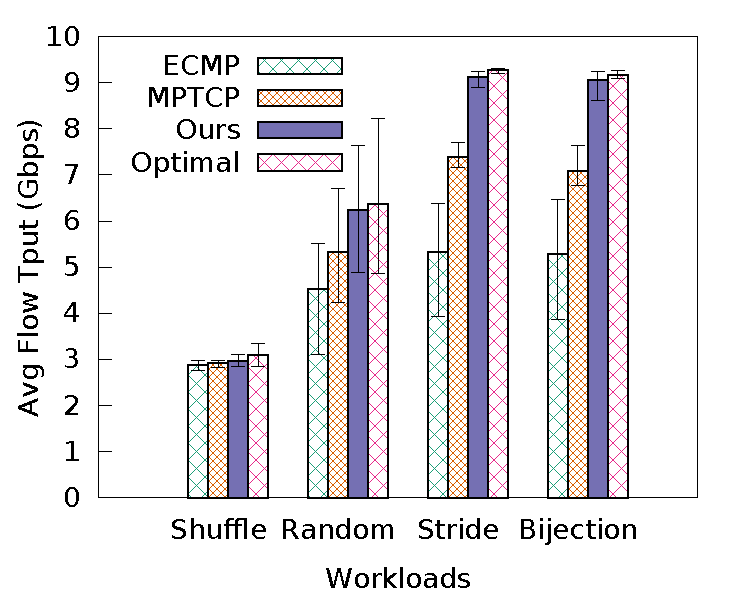
\includegraphics[width=\textwidth]{./figures/macro/stride/macro_compare_tput_witherrbar.pdf}
                \caption{}
                \label{tput}
        \end{subfigure}
        \begin{subfigure}[b]{0.225\textwidth}
                \centering
                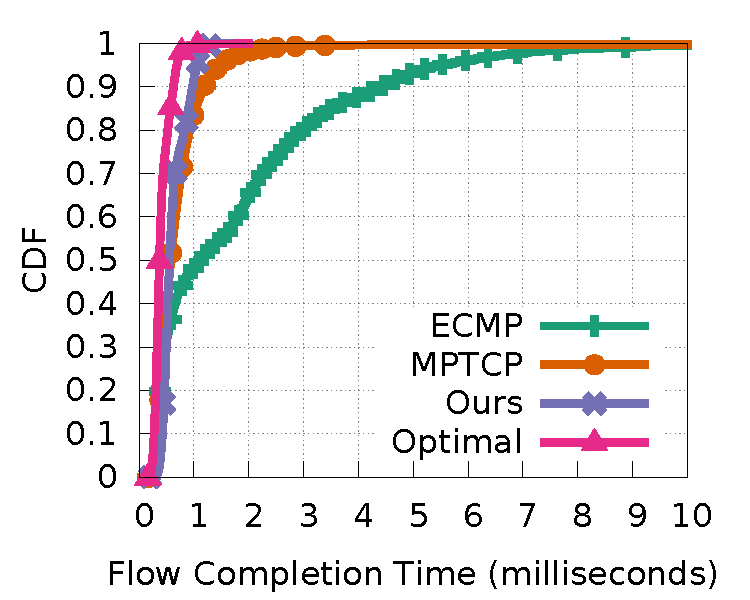
\includegraphics[width=\textwidth]{./figures/macro/bijection/macro_compare_fct_bijection_mice.pdf}
                \caption{}
                \label{fct}
        \end{subfigure}
        \caption{System performance (a) elephant flow throughput and (b) mice flow (50KB) completion time.}
        \label{performance}
\end{figure}


We conducted experiments on a physical
testbed consisting of 16 servers and a 2-tier Clos network with 8 10G switches. 
Then we compared our approach with ECMP, MPTCP and Optimal (\ie{}, all the servers are connected to a non-blocking switch) using several workloads.
Figure~\ref{performance} shows that our load balancing scheme outperforms existing ones and closely track that of Optimal.
\section{Conclusion}
We present a near uniform sub-flow distributed load balancing scheme
that can near optimally load balance the network at high networking speeds.
Our scheme makes a few simple changes to the hypervisor soft-edge (vSwitch and GRO)
and does not require any modifications to the transport layer or network hardware.
